\documentclass[12pt]{article}

\usepackage{algorithm}
\usepackage{algpseudocode}
\usepackage{amsmath}
\usepackage{amsfonts}
\usepackage{float}
\usepackage{fancyhdr}
\usepackage{graphicx}
\usepackage{placeins}
\usepackage[colorlinks=true,linkcolor=blue, citecolor=red]{hyperref}
\usepackage{url}
\usepackage[top=.75in, left=.75in, right=.75in, bottom=1in]{geometry}
\usepackage{arydshln}
\usepackage[utf8]{vietnam}
\setlength{\headheight}{29.43912pt}

\usepackage{mathptmx}
% \graphicspath{PATH_TO_GRAPHIC_FOLDER}

\pagestyle{fancy}
\fancyfoot{}
\fancyfoot[R]{Page \thepage}

\lhead{
Báo cáo đồ án môn học
}
\rhead{
Trường Đại học Khoa học Tự nhiên - ĐHQG HCM\\
Khai thác ngữ liệu văn bản nâng cao (MTH089)
}
\lfoot{\LaTeX\ template by \href{https://github.com/trhgquan}{Quan, Tran Hoang}}

\newcommand{\coursename}{Khai thác ngữ liệu văn bản nâng cao (MTH089)}
\newcommand{\reportname}{ViHealthBERT: Pre-trained Language Models for Vietnamese in Health Text Mining}

\begin{document}

\begin{titlepage}
\newcommand{\HRule}{\rule{\linewidth}{0.5mm}}
\centering

\textsc{\LARGE đại học quốc gia tphcm}\\[1.5cm]
\textsc{\Large trường đại học khoa học tự nhiên}\\[0.5cm]
\textsc{\large khoa công nghệ thông tin}\\[0.5cm]
% \textsc{bộ môn công nghệ tri thức}\\[0.5cm]

\HRule \\[0.4cm]
{ 
\huge{\bfseries{Báo cáo Seminar}}\\[0.5cm]
\large{\bfseries{Đề tài: \reportname}}
}\\[0.4cm]
\HRule \\[0.5cm]

\textbf{\large Môn học: \coursename}\\[0.5cm]

\begin{minipage}[t]{0.4\textwidth}
\begin{flushleft} \large
\emph{Học viên thực hiện:}\\
Trần Hoàng Quân (19120338) \\
Phạm Anh Việt \textsc{(20C11060)} \\
Nguyễn Đức Thuận \textsc{(21C11035)} \\
Nguyễn Thiện Dương \textsc{(21C12004)} \\
\end{flushleft}
\end{minipage}
~
\begin{minipage}[t]{0.4\textwidth}
\begin{flushright} \large
\emph{Giáo viên hướng dẫn:} \\
% Dr. James \textsc{Smith}
TS. Nguyễn Trường Sơn\\
TS. Nguyễn Tiến Huy
\end{flushright}
\end{minipage}\\[1cm]

{\large \today}\\[1cm]


\includegraphics[scale=.3]{img/hcmus-logo.png}\\[1cm] 

\vfill
\end{titlepage}


\tableofcontents
\pagebreak

\section{Tóm tắt nội dung bài báo}
Trong những năm gần đây, các mô hình ngôn ngữ (Language Models - LM) được xây dựng và ứng dụng rộng rãi trong lĩnh vực Xử lý ngôn ngữ tự nhiên (NLP), chúng cũng đạt được nhiều kết quả đáng chú ý. Đặc biệt, chất lượng các mô hình đơn ngữ được huấn luyện sẵn dành cho những ngôn ngữ ít tài nguyên ngữ liệu đã tăng đáng kể. Đáng lưu ý, mặc dù các mô hình ngôn ngữ cho miền chung (general-domain language models) rất đa dạng, nhưng có rất ít các mô hình ngôn ngữ đặc thù dành riêng cho một số lĩnh vực (specific-domain language models). Vì lí do đó, nhóm tác giả bài báo \textit{ViHealthBERT: Pre-trained Language Models for Vietnamese in Health Text Mining}\cite{minh-EtAl:2022:LREC} công bố bài báo với những đóng góp sau:
\begin{itemize}
\item Giới thiệu mô hình ViHealthBERT là mô hình ngôn ngữ Tiếng Việt đặc thù cho lĩnh vực y tế.
\item Giới thiệu các bộ ngữ liệu Acronym Disambiguation (AD) và Freqently Asked Question (FAQ) Summarization là các bộ ngữ liệu đặc thù cho lĩnh vực y tế.
\end{itemize}

\section{Kiến trúc mô hình ViHealthBERT}
\subsection{Transformer và BERT}
Mô hình Transformer ứng dụng cơ chế self-attention và multi-head attention được giới thiệu lần đầu trong paper Attention is All You Need\cite{DBLP:journals/corr/VaswaniSPUJGKP17}. 
\begin{figure}
\centering
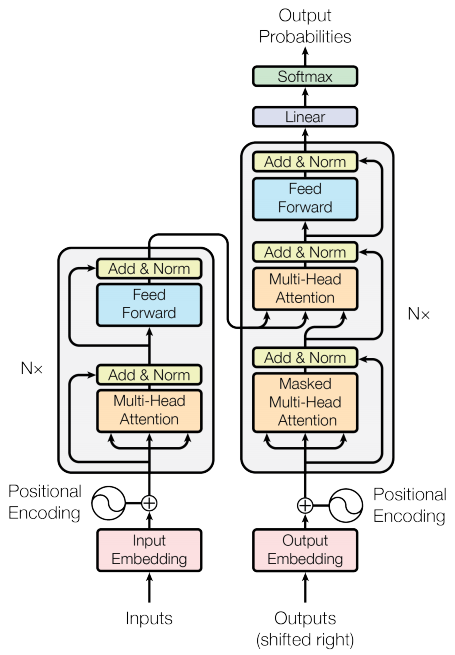
\includegraphics[scale=.35]{img/transformer.png}
\caption{Kiến trúc Transformer\cite{DBLP:journals/corr/VaswaniSPUJGKP17}}
\label{fig:transformer_diagram}
\end{figure}
Phần Encoder của Transformer được sử dụng trong mô hình BERT (\textbf{B}idirectional \textbf{E}ncoder \textbf{R}epresentations from \textbf{T}ransformers)\cite{devlin-etal-2019-bert}. Trong bài báo, BERT được giới thiệu có 2 phiên bản với các siêu tham số (hyperparameters) và số lượng tham số huấn luyện (training parameters) khác nhau:
\begin{itemize}
\item \textbf{BERT\textsubscript{base}}: 12 Transformer encoder layers, 768 hidden units, 12 attention heads, 110 triệu parameters.
\item \textbf{BERT\textsubscript{large}}: 24 Transformer encoder layers, 1024 hidden units, 16 attention heads và 340 triệu parameters.
\end{itemize}
\begin{figure}
\centering
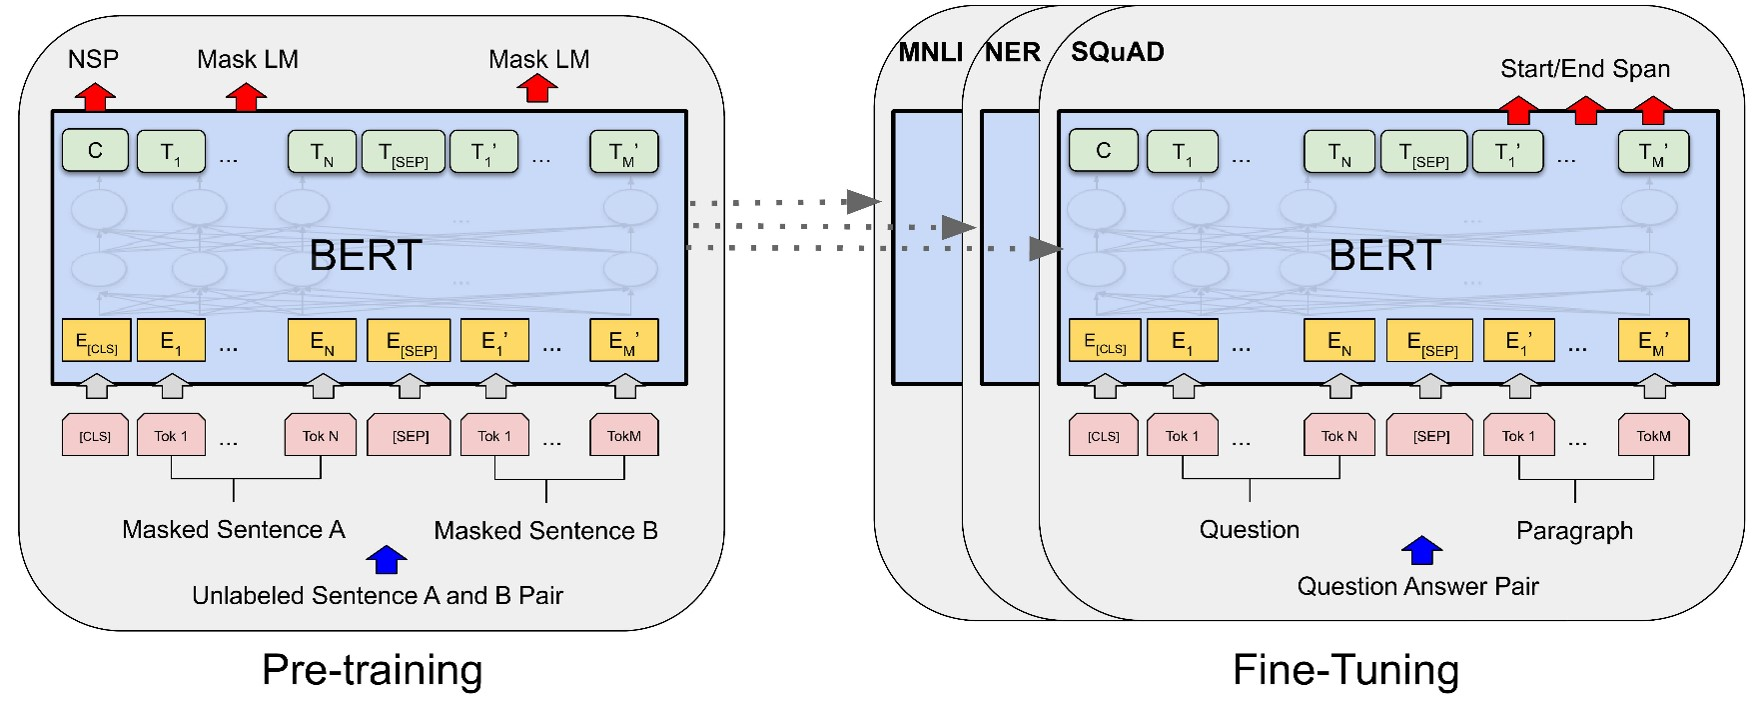
\includegraphics[scale=.65]{img/BERT.jpg}
\caption{Mô hình BERT\cite{devlin-etal-2019-bert}}
\label{fig:my_label}
\end{figure}
BERT được tiền huấn luyện (pretraining) với bộ ngữ liệu \textit{BookCorpus} (800 triệu từ) và \textit{Wikipedia English} (2500 triệu từ), sau đó tinh chỉnh (finetune) lại cho từng task khác nhau. Sau khi BERT được công bố, nhiều mô hình cải tiến của BERT cũng được giới thiệu dựa trên kiến trúc của BERT, trong đó có thể kể đến
\begin{itemize}
\item \textbf{RoBERTa} (\textbf{R}obustly \textbf{o}ptimized \textbf{BERT} Pretraining \textbf{a}pproach)\cite{DBLP:journals/corr/abs-1907-11692}: sử dụng dynamic masking so với sử dụng static masking trong kiến trúc gốc; huấn luyện trên nhiều ngữ liệu hơn.
\item \textbf{DistilBERT}\cite{DBLP:journals/corr/abs-1910-01108}: mô hình nhỏ, nhanh, tốn ít chi phí huấn luyện hơn mô hình BERT gốc: có ít hơn 40\% parameters, chạy nhanh hơn 60\% nhưng hiệu quả bằng 95\% so với mô hình gốc.
\end{itemize}

\subsection{PhoBERT}
Dựa trên mô hình BERT, nhóm nghiên cứu từ VinAI đã công bố PhoBERT\cite{phobert}, được giới thiệu là mô hình ngôn ngữ đơn ngữ dành cho tiếng Việt có quy mô lớn đầu tiên. PhoBERT sử dụng quá trình pretraining của RoBERTA để tăng hiệu quả cho mô hình. Kiến trúc của PhoBERT vẫn giữ nguyên so với BERT:
\begin{itemize}
\item \textbf{PhoBERT\textsubscript{base}}: 12 encoder layers, 768 hidden units, 12 attention heads, 135 triệu parameters.
\item \textbf{PhoBERT\textsubscript{large}}: 24 encoder layers, 1024 hidden units, 16 attention heads và 370 triệu parameters.
\end{itemize}
PhoBERT được pretrain với bộ ngữ liệu \textit{Wikipedia Tiếng Việt} và bộ ngữ liệu tin tức tiếng Việt \textit{Binhvq News Corpus}

\subsection{ViHealthBERT}
Mô hình ViHealthBERT sử dụng kiến trúc của BERT (12 encoder layer, 768 hidden units, 12 attention heads) với bộ trọng số huấn luyện của PhoBERT. Việc huấn luyện ViHealthBERT chia làm 2 giai đoạn:
\begin{itemize}
\item \textbf{Giai đoạn pretraining}: Huấn luyện trên các bộ ngữ liệu \textit{Text Mining Corpus} và \textit{OSCAR} : Masked Language Modeling (MLM), Capitalized Prediction (CP) và Next Sentence Prediction (NSP).
\item \textbf{Giai đoạn finetuning}: Finetuning trên các bộ ngữ liệu \textit{PhoNER\_COVID-19, VimQ, arcDrid} và \textit{FAQ Summarization}: Named-Entity Recognition (NER), Acronym Disambiguation và FAQ Summarization
\end{itemize}
\begin{figure}
\begin{center}
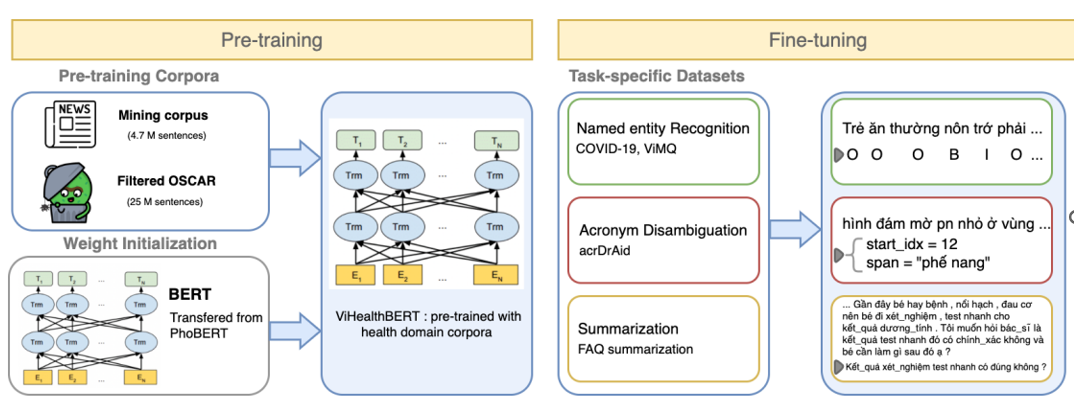
\includegraphics[scale=.8]{img/ViHealthBERT.png}
\caption{Tổng quan về quá trình pretraining và finetuning trong ViHealthBERT\cite{minh-EtAl:2022:LREC}}
\end{center}
\end{figure}

\section{Ngữ liệu huấn luyện}

\section{Demo}

% \cleardoublepage
\phantomsection
\addcontentsline{toc}{section}{Tài liệu}
\bibliographystyle{apalike}
\bibliography{sample}

\end{document}